\documentclass{article}
\usepackage[utf8]{inputenc}
\usepackage{vmargin}


\usepackage{amsmath} 
\usepackage{graphicx}
\usepackage{graphics}
\usepackage{float}
\usepackage{blindtext}
\usepackage{listings}
\usepackage{xcolor}
\usepackage[spanish]{babel}
\usepackage{subfig}

\graphicspath{ {images/} }
\title{Ondas Fisica Computacional}
\date{}
\setpapersize{A4}
\setmargins{2.5cm}       % margen izquierdo
{1.5cm}                        % margen superior
{16.5cm}                      % anchura del texto
{23.42cm}                    % altura del texto
{10pt}                           % altura de los encabezados
{1cm}                           % espacio entre el texto y los encabezados
{0pt}                             % altura del pie de página
{2cm}                           % espacio entre el texto y el pie de página

\begin{document}

%-------COLORES PARA CODIGO ------------------------
\lstdefinestyle{customc}{
  belowcaptionskip=1\baselineskip,
  breaklines=true,
  frame=L,
  xleftmargin=\parindent,
  language=JavaScript,
   basicstyle=\footnotesize\ttfamily,
  showstringspaces=false,
  basicstyle=\footnotesize\ttfamily,
  keywordstyle=\bfseries\color{green!40!black},
  commentstyle=\itshape\color{purple!40!black},
  identifierstyle=\color{blue},
  stringstyle=\color{orange},
  frame=single,	  
  numbers=left,
   numberstyle=\footnotesize,
}

\lstdefinestyle{customasm}{
  belowcaptionskip=1\baselineskip,
  frame=L,
  xleftmargin=\parindent,
  language=JavaScript,
  basicstyle=\footnotesize\ttfamily,
  commentstyle=\itshape\color{purple!40!black},
}

\lstset{escapechar=@,style=customc}

%---------------------------------------------

\thispagestyle{empty}

\vfill
 \begin{center}
    \begin{figure}[h]
    \centering
    \includegraphics[width=12cm]{unsa}\\
    
    \end{figure}
 	 
     \vspace*{1.5cm}
    {\large\bfseries FACULTAD DE PRODUCCIÓN Y SERVICIOS} \\
    {\large\bfseries ESCUELA PROFESIONAL DE CIENCIA DE LA COMPUTACIÓN}  \\    
    \vspace*{1.5cm}
    
 	\rule[0.5ex]{\linewidth}{2pt}\vspace*{-\baselineskip}\vspace*		{3.2pt}
	\rule[0.5ex]{\linewidth}{1pt}\\[\baselineskip]
 	{\huge Física Computacional} \\[4mm]
    \rule[0.5ex]{\linewidth}{1pt}\vspace*{-							\baselineskip}\vspace{3.2pt}
	\rule[0.5ex]{\linewidth}{2pt}\\
 	\vspace*{1cm}

    \begin{large} \bfseries
    Práctica 7: Ondas \\
    
    \vspace{5mm}
    Eduardo Antonio Sánchez Hincho \\

    \vspace{5mm}
    Docente:\\
    Edwin Agapito Llamoca Requena
    \end{large}
    \vspace*{0.4in}
    
    \noindent \\
    
    \vfill
    \large\bfseries{ AREQUIPA\\2020}
\end{center}
\newpage

\section{ Solución aproximada de la ecuación de Onda}
Primero veremos como se ejecutó con las condiciones iniciales del problema, el código fue el siguiente:
\begin{lstlisting}[language=octave,caption=onda.m]
function U=onda(f,g,a,b,v,h,k)
% f es la condici´on inicial de la posici´on
% g es la condici´on inicial de la velocidad
% v es la velocidad de propagaci´on de la onda
% a es la longitud de la cuerda
% b es la tiempo que se necesita para evaluar la onda
% h es la tama~no de paso para el espacio
% k es la tama~no de paso para el tiempo
% U es la matriz donde se almacena la solucion numerica
n=a/h+1;
m=b/k+1;
% r es calculo para la condicion de estabilidad
r=v*k/h;
r1=r^2;
r2=r^2/2;
s1=1-r^2;
s2=2*(1-r^2);
U=zeros(n,m);
% calculo de las primeras dos filas
for i=2:n-1
  U(i,1)=feval(f,h*(i-1));
  U(i,2)=s1*feval(f,h*(i-1))+k*feval(g,h*(i-1))+r2*(feval(f,h*i)+feval(f,h*(i-2)));
end
% calculo a partir de la tercera fila
for j=2:m-1
  for i=2:n-1
      U(i,j+1)= s2*U(i,j)+r1*(U(i-1,j)+U(i+1,j))-U(i,j-1);
  end
  surfc(U)
end
\end{lstlisting}
\begin{lstlisting}[language=octave,caption=fx.m]
function y=f(x)
  y=x^2-x+sin(2*pi*x)
endfunction
\end{lstlisting}
\begin{lstlisting}[language=octave,caption=gx.m]
function y=g(x)
  y=0;
endfunction
\end{lstlisting}
El resultado fue el siguiente con h=0.05, k=0.01 y v=2.
\begin{figure}[H]
    \centering
    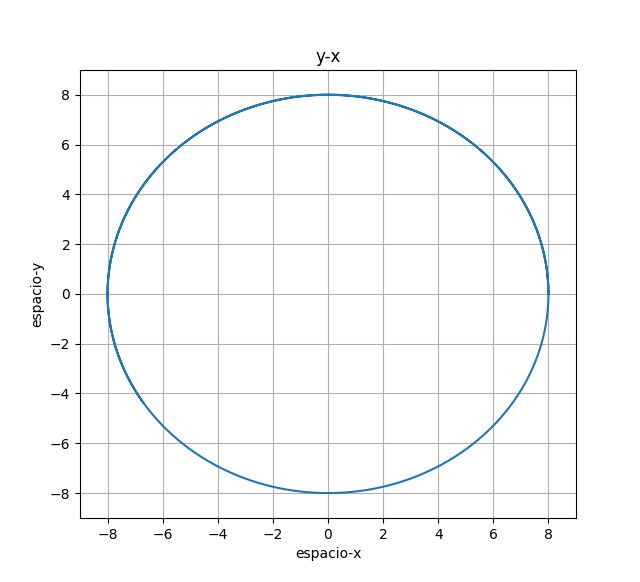
\includegraphics[width=0.8\textwidth]{1.png}
    \caption{Gráfica}
\end{figure}
\subsection{Analice el mismo problema, cambiando h y k y verifique sus resultados}
Se cambio los valores por:\\
$
h = 0.04\\
k = 0.02\\
v = 1\\
$
Se obtuvo la siguiente gráfica:
\begin{figure}[H]
    \centering
    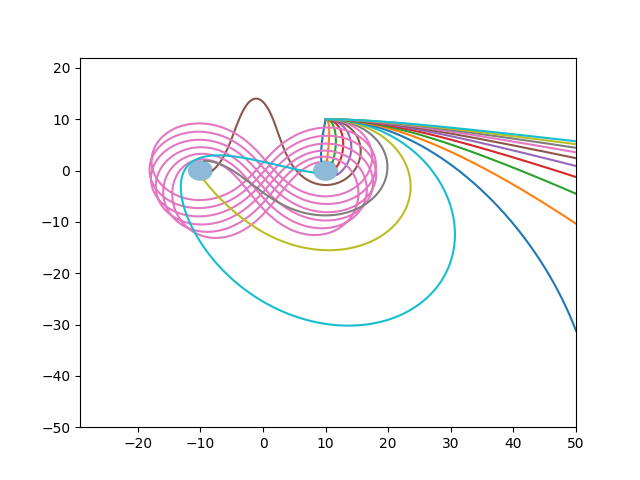
\includegraphics[width=0.8\textwidth]{2.png}
    \caption{Gráfica}
\end{figure}
Como vemos, ahora se generaron menos ondas en el gráfico

\subsection{Verifique que si no cumple r \leq 1, como se verían los resultados ?}
Se cambiaran los valor de v,h y k por:
$
h = 0.04\\
k = 0.05\\
v = 4\\
$
Obteniendo los siguientes resultados, para r = 5
\begin{figure}[H]
    \centering
    \includegraphics[width=0.8\textwidth]{3.png}
    \caption{Gráfica}
\end{figure}
Este fue el resultado final, pero en el gif mandado, se observara los resultados mas a detalle de como poco a poco fue cambiando. Al no cumplir la condición de r \leq 1, los resultados se vuelven inestables, como podemos observar, y ya no vemos ondas.

\section{Problema desafío}
\subsection{}
Se cambio la función f(x) según lo indicado por el problema
\begin{lstlisting}[language=octave,caption=fx2.m]
function y=fx2(x)
  if (x>=0 && x<=0.5)
    y=2*x;
  end
  if (x>=0.5 && x<=1)
    y=2-2*x;
  end
endfunction
\end{lstlisting}
Se pasaron los valores h y k dados por el problema, y se cambio la v a 1. Se obtuvo el siguiente resultado:
\begin{figure}[H]
    \centering
    \includegraphics[width=0.8\textwidth]{4.png}
    \caption{Gráfica}
\end{figure}
\subsection{}
Para este problema, se adicionó el siguiente código al archivo onda.m, esto para mostrar en subplots de 10 en 10, como fue la transformación.
\begin{lstlisting}[language=octave,caption=onda.m]
for k=11:10:101
  subplot(5,2,(k-1)/10 );
  plot(U(:,k));
end
\end{lstlisting}
Se obtuvo lo siguiente:
\begin{figure}[H]
    \centering
    \includegraphics[width=1\textwidth]{5.png}
    \caption{Gráfica}
\end{figure}

\end{document}
